\FloatBarrier
\chapter{Results} \lhead{\emph{Results}}

\section{Results on the benchmark systems}

\subsection{Noiseless data}

These are the results for the trajectories generated from the noiseless Lorenz systems described in section \ref{sec:noiseless_lorenz}.
For the analysis, I chose the models trained for 1000 epochs. I treated a model run as not converged if the 
$D_{stsp}$ is larger than 1. Those runs were not included in the quantitative analysis summarized in table \ref{tab:noiseless_comp_table}. The distributions 
of the state space divergence and the power spectrum error are additionally displayed in figures \ref{fig:Comparison_D_stsp_noiseless} and \ref{fig:Comparison_D_PSE_noiseless}. 
The non-convergent runs are grouped together at $-0.2$ on the histograms, thereby constraining the range of bins to enhance visualization.

The results overall are as intended. On the unconvoluted dataset, the linear observation model performs better while on the convolutional datasets the convolutional
observation model outperforms. The performance disparity grows with decreased repeat time as a lower repeat time degrades the Lorenz attractor more heavily. It is noticeable 
for both models that the number of failed model runs increases with a stronger degradation of the observed trajectories. At $hrf_{0.2}$ the linear model doesn't converge
reliably at all anymore (defined as $D_{stsp}<1$). Reviewing the training in this case shows a lack of stability. There are individual epochs with good fits, but the model 
never converges there, but jumps back to a worse fit a few training epochs later. This is showcased qualitatively in figure \ref{fig:traj_gen_3d}.

\begin{figure}
    \includegraphics[width=\textwidth]{Images/Comparison_D_stsp_noiseless.png}
    \caption[Comparison of $D_{stsp}$ noiseless]{\textbf{Comparison of $D_{stsp}$ noiseless: } Distributions of $D_{stsp}$ of the convolutional observation model
    and the linear identity model. The bins at -0.2 are the model runs which did not converge, which is defined as models with $D_{stsp}>1$.}
    \label{fig:Comparison_D_stsp_noiseless}
\end{figure}

\begin{figure}
    \includegraphics[width=\textwidth]{Images/Comparison_D_PSE_noiseless.png}
    \caption[Comparison of $D_{PSE}$ noiseless]{\textbf{Comparison of $D_{PSE}$ noiseless: } Distributions of $D_{PSE}$ of the convolutional observation model
    and the linear identity model. The bins at -0.2 are the model runs which did not converge, which is defined as models with $D_{stsp}>1$.}
    \label{fig:Comparison_D_PSE_noiseless}
\end{figure}

\begin{table}
\caption{Quantitative comparison between linear and convolutional observation model}
\label{tab:noiseless_comp_table}
\begin{tabular}{llllll}
\toprule
Dataset & Obs model & $N_{converged}$ & 20 step PE & $D_{stsp}$ & $D_{PSE}$ \\
\midrule
Unconv & Lin & 92 & $0.0004 \pm 0.0001$ & $0.09 \pm 0.02$ & $0.06 \pm 0.01$ \\
Unconv & Conv & 94 & $0.0004 \pm 0.0001$ & $0.09 \pm 0.03$ & $0.05 \pm 0.01$ \\
$hrf_{1.2}$ & Lin & 87 & $0.0006 \pm 0.0001$ & $0.09 \pm 0.02$ & $0.05 \pm 0.02$ \\
$hrf_{1.2}$ & Conv & 88 & $0.0007 \pm 0.0001$ & $0.09 \pm 0.02$ & $0.05 \pm 0.01$ \\
$hrf_{0.5}$ & Lin & 83 & $0.0105 \pm 0.0016$ & $0.27 \pm 0.14$ & $0.08 \pm 0.03$ \\
$hrf_{0.5}$ & Conv & 90 & $0.0009 \pm 0.0001$ & $0.11 \pm 0.07$ & $0.07 \pm 0.02$ \\
$hrf_{0.2}$ & Lin & 0 & $- \pm -$ & $- \pm -$ & $- \pm -$ \\
$hrf_{0.2}$ & Conv & 63 & $0.0028 \pm 0.0004$ & $0.35 \pm 0.14$ & $0.11 \pm 0.04$ \\
\bottomrule
\end{tabular}
\end{table}


\begin{figure}
    \centering
    \begin{subfigure}[b]{0.24\textwidth}
        \centering
        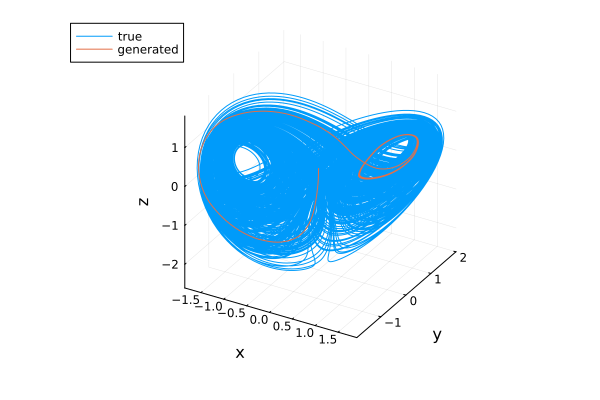
\includegraphics[width=\linewidth]{Images/training_epochs/traj_gen_3d_125.png}
        \caption{At epoch 125}
        \label{fig:traj_gen_3d_125}
    \end{subfigure}%
    \begin{subfigure}[b]{0.24\textwidth}
        \centering
        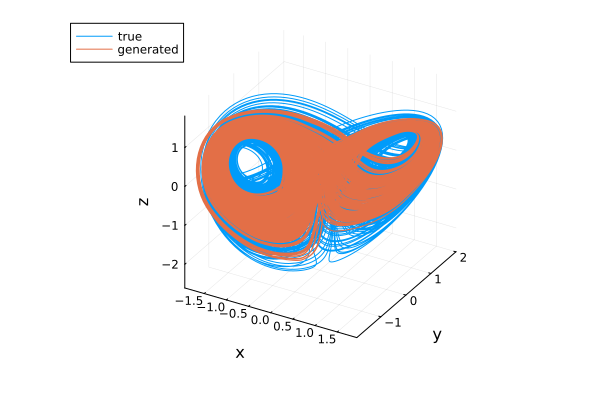
\includegraphics[width=\linewidth]{Images/training_epochs/traj_gen_3d_150.png}
        \caption{At epoch 150}
        \label{fig:traj_gen_3d_150}
    \end{subfigure}%
    \begin{subfigure}[b]{0.24\textwidth}
        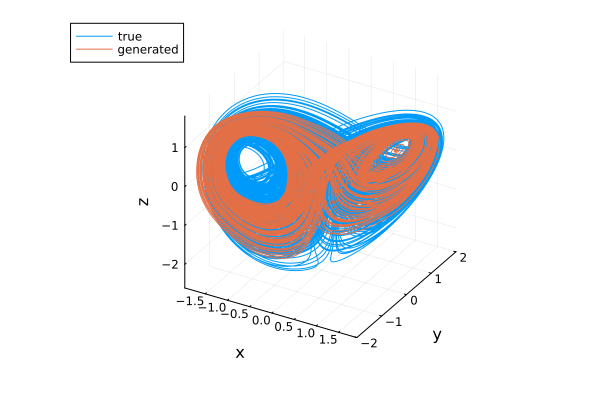
\includegraphics[width=\textwidth]{Images/training_epochs/traj_gen_3d_175.png}
        \caption{At epoch 175}
        \label{fig:traj_gen_3d_175}
    \end{subfigure}%
    \begin{subfigure}[b]{0.24\textwidth}
        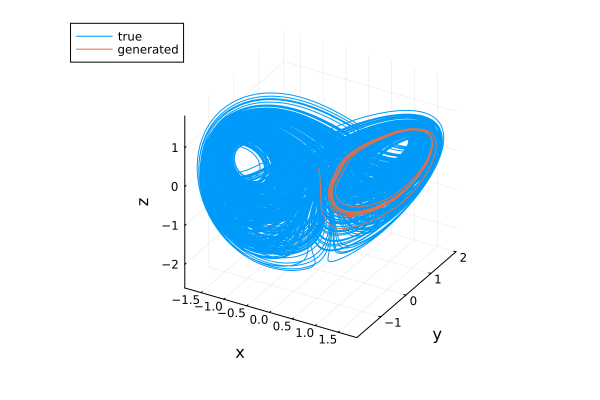
\includegraphics[width=\textwidth]{Images/training_epochs/traj_gen_3d_200.png}
        \caption{At epoch 200}
        \label{fig:traj_gen_3d_200}
    \end{subfigure}
       \caption[Training instability in the presence of strong convolution]{\textbf{Training instability in the presence of strong convolution: } Trajectories of the training data 
       (a Lorenz attractor convoluted with an $hrf_{0.2}$) and of the model with linear observation equation at different training epochs.}
       \label{fig:traj_gen_3d}
\end{figure}
   
\subsection{Noisy data}

These are the results for the trajectories generated from the noisy Lorenz systems described in section \ref{sec:noisy_lorenz}. 
For the analysis, I chose the models trained for 1000 epochs. I treated a model run as not converged if the 
$D_{stsp}$ is larger than 1. Those runs were not included in the quantitative analysis summarized in table \ref{tab:noisy_comp_table}. The distributions 
of the metrics, state space divergence, power spectrum error and 20-step prediction error (PE), in the case of $hrf_{0.5}$ are additionally displayed
in figure \ref{fig:Comparison_hrf_0_5_noisy}. The non-convergent runs are grouped together at $-0.2$ on the histograms, 
thereby constraining the range of bins to enhance visualization.

The results are analogous to the noiseless case. The stronger the degradation of the underlying trajectories by both noise and convolution, the better the convolutional
observation model performs compared to the linear.

   
\begin{figure}
    \includegraphics[width=\textwidth]{Images/Comparison_hrf_0_5_noisy.png}
    \caption[Comparison of performance metrics on dataset convoluted with $hrf_{0.5}$ and added white noise]
    {\textbf{Comparison of performance metrics on dataset convoluted with $hrf_{0.5}$ and added white noise: } Distributions of $D_{PSE}$ and $D_{stsp}$ of the convolutional observation model
    and the linear identity model. The bins at -0.2 are the model runs which did not converge, which is defined as models with $D_{stsp}>1$.}
    \label{fig:Comparison_hrf_0_5_noisy}
\end{figure}

\begin{table}
\caption{Quantitative comparison between linear and convolutional observation model on noisy data}
\label{tab:noisy_comp_table}
\begin{tabular}{lllllll}
\toprule
Convolution & $\sigma$ & Obs model & $N_{converged}$ & 20 step PE & $D_{stsp}$ & $D_{PSE}$ \\
\midrule
$hrf_{1.2}$ & 0.01 & Lin & 78 & $0.0013 \pm 0.0001$ & $0.10 \pm 0.10$ & $0.05 \pm 0.01$ \\
$hrf_{1.2}$ & 0.01 & Conv & 80 & $0.0011 \pm 0.0001$ & $0.09 \pm 0.02$ & $0.06 \pm 0.01$ \\
$hrf_{0.5}$ & 0.01 & Lin & 84 & $0.0114 \pm 0.0014$ & $0.27 \pm 0.14$ & $0.09 \pm 0.03$ \\
$hrf_{0.5}$ & 0.01 & Conv & 90 & $0.0012 \pm 0.0001$ & $0.09 \pm 0.02$ & $0.06 \pm 0.01$ \\
$hrf_{0.2}$ & 0.01 & Lin & 1 & $0.0283 \pm 0.0000$ & $0.93 \pm 0.00$ & $0.19 \pm 0.00$ \\
$hrf_{0.2}$ & 0.01 & Conv & 90 & $0.0023 \pm 0.0001$ & $0.22 \pm 0.04$ & $0.14 \pm 0.02$ \\
$hrf_{1.2}$ & 0.1 & Lin & 86 & $0.0387 \pm 0.0002$ & $0.45 \pm 0.02$ & $0.09 \pm 0.01$ \\
$hrf_{1.2}$ & 0.1 & Conv & 85 & $0.0158 \pm 0.0001$ & $0.44 \pm 0.02$ & $0.09 \pm 0.01$ \\
$hrf_{0.5}$ & 0.1 & Lin & 92 & $0.0538 \pm 0.0015$ & $0.46 \pm 0.03$ & $0.10 \pm 0.01$ \\
$hrf_{0.5}$ & 0.1 & Conv & 84 & $0.0145 \pm 0.0001$ & $0.41 \pm 0.02$ & $0.09 \pm 0.01$ \\
$hrf_{0.2}$ & 0.1 & Lin & 2 & $0.0813 \pm 0.0007$ & $0.97 \pm 0.01$ & $0.18 \pm 0.00$ \\
$hrf_{0.2}$ & 0.1 & Conv & 84 & $0.0191 \pm 0.0002$ & $0.70 \pm 0.08$ & $0.24 \pm 0.02$ \\
\bottomrule
\end{tabular}
\end{table}


\FloatBarrier
\section{Grid search on LEMON dataset} \label{sec:results_gridsearch} 

I compiled the results of the hyperparameter search in the following tables and figures. Figure \ref{fig:grid_seach_latent_dimension} shows the mean and standard deviation
for varying the latent dimension $\ell$. The quantitative results are also displayed in table \ref{tab:gridsearch_ldim_table}. The results show that the model performs similarly 
for all the different tested $\ell$-values. The largest differences in performance are seen in the $D_{stsp}$ values. The value $\ell = 16$ has by far the lowest variation in 
$D_{stsp}$ across both train and test set. Hence, I chose $\ell=16$ as the value for training on the entire dataset.

Figure \ref{fig:grid_search_tf_alpha} shows the mean and standard deviation
for varying the teacher forcing $\alpha$. The quantitative results are also displayed in table \ref{tab:gridsearch_alpha_table}. The results are not very straightforward to
interpret. $D_{stsp}$-value improve for very low (or even 0) $\alpha$-values. $D_{PSE}$ is higher at low $\alpha$-values and is lowest $\alpha = 0.1$. The prediction errors 
are also the lowest around $\alpha=0.1$, hence I chose that $\alpha$-value for training on the entire dataset.

\begin{table}
\centering
\caption{Results of the parameter search for $\ell$ values. Model runs where excluded if the 1-step PE $>$ 1}
\label{tab:gridsearch_ldim_table}
\begin{tabular}{rrllllll}
\toprule
$\ell$ & $N_{converged}$ & Dataset & 1-step PE & 5-step PE & 10-step PE & $D_{stsp}$ & $D_{PSE}$ \\
\midrule
8 & 247 & Train & $0.16 \pm 0.14$ & $0.77 \pm 0.64$ & $0.93 \pm 0.53$ & $5.90 \pm 8.61$ & $0.35 \pm 0.11$ \\
8 & 247 & Test & $0.26 \pm 0.17$ & $1.44 \pm 0.66$ & $1.96 \pm 0.54$ & $9.85 \pm 9.67$ & $0.20 \pm 0.08$ \\
12 & 244 & Train & $0.16 \pm 0.15$ & $0.75 \pm 0.72$ & $0.87 \pm 1.14$ & $3.87 \pm 3.76$ & $0.32 \pm 0.11$ \\
12 & 244 & Test & $0.25 \pm 0.18$ & $1.46 \pm 0.60$ & $1.95 \pm 1.02$ & $7.86 \pm 5.21$ & $0.19 \pm 0.07$ \\
16 & 226 & Train & $0.20 \pm 0.20$ & $0.77 \pm 0.77$ & $0.78 \pm 0.54$ & $3.08 \pm 2.08$ & $0.30 \pm 0.10$ \\
16 & 226 & Test & $0.32 \pm 0.25$ & $1.53 \pm 0.67$ & $1.89 \pm 0.51$ & $6.86 \pm 3.13$ & $0.18 \pm 0.08$ \\
20 & 245 & Train & $0.28 \pm 0.17$ & $1.36 \pm 1.44$ & $1.40 \pm 1.48$ & $4.49 \pm 4.77$ & $0.34 \pm 0.12$ \\
20 & 245 & Test & $0.36 \pm 0.22$ & $1.88 \pm 1.44$ & $2.11 \pm 1.50$ & $8.71 \pm 7.05$ & $0.21 \pm 0.08$ \\
24 & 241 & Train & $0.25 \pm 0.15$ & $1.17 \pm 0.95$ & $1.25 \pm 0.69$ & $4.47 \pm 4.08$ & $0.34 \pm 0.13$ \\
24 & 241 & Test & $0.32 \pm 0.19$ & $1.66 \pm 1.04$ & $1.92 \pm 0.61$ & $8.95 \pm 7.45$ & $0.21 \pm 0.10$ \\
\bottomrule
\end{tabular}
\end{table}


\begin{figure}
    \includegraphics[width=\textwidth]{Images/grid_seach_latent_dimension.png}
    \caption[Grid search over latent dimension $ \ell $]
    {\textbf{Grid search over latent dimension $ \ell $: } Mean and standard deviation for the different metrics depending on the latent dimension $\ell$. Model runs 
    where excluded if the 1-step PE $>$ 1}
    \label{fig:grid_seach_latent_dimension}
\end{figure}

\begin{table}
\centering
\caption{Results of the parameter search for $\alpha$ values. Model runs where excluded if the 1-step PE $>$ 1}
\label{tab:gridsearch_alpha_table}
\begin{tabular}{rrllllll}
\toprule
$\alpha$ & $N_{converged}$ & Dataset & 1-step PE & 5-step PE & 10-step PE & $D_{stsp}$ & $D_{PSE}$ \\
\midrule
0.00 & 221 & Train & $0.29 \pm 0.15$ & $1.05 \pm 1.09$ & $1.26 \pm 1.76$ & $2.55 \pm 0.45$ & $0.39 \pm 0.09$ \\
0.00 & 221 & Test & $0.41 \pm 0.24$ & $1.31 \pm 1.02$ & $1.58 \pm 1.71$ & $4.70 \pm 1.45$ & $0.29 \pm 0.08$ \\
0.01 & 247 & Train & $0.31 \pm 0.15$ & $1.63 \pm 1.13$ & $1.42 \pm 0.70$ & $2.50 \pm 0.45$ & $0.32 \pm 0.10$ \\
0.01 & 247 & Test & $0.43 \pm 0.19$ & $2.26 \pm 1.27$ & $2.25 \pm 0.77$ & $4.98 \pm 1.64$ & $0.20 \pm 0.05$ \\
0.03 & 244 & Train & $0.26 \pm 0.17$ & $1.13 \pm 0.92$ & $1.03 \pm 0.31$ & $2.65 \pm 0.92$ & $0.27 \pm 0.09$ \\
0.03 & 244 & Test & $0.34 \pm 0.17$ & $1.81 \pm 0.81$ & $2.08 \pm 0.46$ & $6.55 \pm 2.52$ & $0.15 \pm 0.05$ \\
0.05 & 247 & Train & $0.20 \pm 0.16$ & $0.84 \pm 0.62$ & $0.87 \pm 0.31$ & $2.96 \pm 1.61$ & $0.26 \pm 0.09$ \\
0.05 & 247 & Test & $0.28 \pm 0.17$ & $1.57 \pm 0.65$ & $2.00 \pm 0.45$ & $8.09 \pm 4.16$ & $0.15 \pm 0.05$ \\
0.10 & 250 & Train & $0.09 \pm 0.06$ & $0.51 \pm 0.26$ & $0.67 \pm 0.27$ & $3.76 \pm 2.77$ & $0.25 \pm 0.08$ \\
0.10 & 250 & Test & $0.16 \pm 0.07$ & $1.25 \pm 0.33$ & $1.84 \pm 0.35$ & $9.59 \pm 4.38$ & $0.14 \pm 0.04$ \\
0.15 & 246 & Train & $0.09 \pm 0.13$ & $0.51 \pm 0.64$ & $0.67 \pm 0.55$ & $5.20 \pm 3.46$ & $0.30 \pm 0.09$ \\
0.15 & 246 & Test & $0.17 \pm 0.18$ & $1.28 \pm 0.66$ & $1.85 \pm 0.50$ & $11.23 \pm 5.32$ & $0.16 \pm 0.05$ \\
0.20 & 246 & Train & $0.09 \pm 0.12$ & $0.44 \pm 0.59$ & $0.69 \pm 0.61$ & $6.88 \pm 6.60$ & $0.34 \pm 0.11$ \\
0.20 & 246 & Test & $0.16 \pm 0.15$ & $1.24 \pm 0.54$ & $1.86 \pm 0.38$ & $12.76 \pm 7.90$ & $0.17 \pm 0.07$ \\
0.25 & 243 & Train & $0.10 \pm 0.15$ & $0.50 \pm 0.74$ & $0.88 \pm 0.95$ & $9.77 \pm 10.69$ & $0.37 \pm 0.11$ \\
0.25 & 243 & Test & $0.18 \pm 0.19$ & $1.33 \pm 0.72$ & $2.05 \pm 0.64$ & $15.32 \pm 10.97$ & $0.18 \pm 0.08$ \\
0.30 & 241 & Train & $0.10 \pm 0.15$ & $0.52 \pm 0.78$ & $0.90 \pm 0.98$ & $10.35 \pm 9.02$ & $0.41 \pm 0.12$ \\
0.30 & 241 & Test & $0.17 \pm 0.17$ & $1.33 \pm 0.63$ & $2.05 \pm 0.60$ & $16.31 \pm 10.90$ & $0.21 \pm 0.09$ \\
\bottomrule
\end{tabular}
\end{table}


\begin{figure}
    \includegraphics[width=\textwidth]{Images/grid_search_tf_alpha.png}
    \caption[Grid search over teacher forcing $\alpha$]
    {\textbf{Grid search over teacher forcing $\alpha$: } Mean and standard deviation for the different metrics depending on the teacher forcing $\alpha$. Model runs 
    where excluded if the 1-step PE $>$ 1}
    \label{fig:grid_search_tf_alpha}
\end{figure}

\FloatBarrier
\section{Analysis of the results on the LEMON dataset} \label{sec:results_main_run}

In this section I have compiled the results of training on the entire filtered (see section \ref{sec:filter_lemon}) LEMON dataset.
For that I trained 20 models on each participant with the hyperparameters $\ell = 16$ and $\alpha=0.1$, the other hyperparameters can be found in \ref{tab:args lemon runs}.

The results of the training are shown in figure \ref{fig:histograms_metrics_main_run}, which shows the distributions of the different metrics on both the training 
and the test datasets. Table \ref{tab:main_run_results} also summarizes these results in terms of mean and standard deviation of the different metrics.
\begin{table}
\centering
\caption{Quantitative Results of the PLRNN with BOLD observation model on the LEMON dataset. Model runs where excluded if the 1-step PE $>$ 1. $N_{converged}=1007$}
\label{tab:main_run_results}
\begin{tabular}{lll}
\toprule
metric & Train Data & Test Data \\
\midrule
$D_{stsp}$ & $2.84 \pm 2.49$ & $8.78 \pm 3.46$ \\
$D_{PSE}$ & $0.21 \pm 0.07$ & $0.14 \pm 0.04$ \\
1-step PE & $0.06 \pm 0.07$ & $0.17 \pm 0.33$ \\
5-step PE & $0.30 \pm 0.26$ & $1.20 \pm 0.41$ \\
10-step PE & $0.41 \pm 0.33$ & $1.78 \pm 0.38$ \\
\bottomrule
\end{tabular}
\end{table}


\begin{figure}
    \includegraphics[width=\textwidth]{Images/histograms_metrics_main_run.png}
    \caption[Distributions of metrics on train and test data]
    {\textbf{Distributions of metrics on train and test data: } Histograms of the results of each model run on the train and test data. Binning of the predictions errors 
    is identical for better visual comparison.}
    \label{fig:histograms_metrics_main_run}
\end{figure}

Looking at the histograms in figure \ref{fig:histograms_metrics_main_run} we can see that results on the test set appear worse overall, having both higher mean and 
higher variation, across all metrics, with the notable exception of $D_{PSE}$ where this relationship appears to be reversed.
I employed the Wilcoxon signed-rank test (method found in \cite{mcdonald2014handbook}, used implementation by \cite{2020SciPy-NMeth}) to establish the statistical
significance of the disparities in metric distributions between the training and test sets. The test results are gathered in table \ref{tab:wilcoxon_test_metrics_train_test}
and as expected the distributions between train and test set all differ significantly.

\begin{table}
\centering
\caption{Wilcoxon signed-rank test applied to the distribution of metrics on training and test set. Model runs where excluded if the 1-step PE $>$ 1. $N_{converged}=1007$}
\label{tab:wilcoxon_test_metrics_train_test}
\begin{tabular}{lllll}
\toprule
 & Result & p-Value & Rank sum & Z-statistic \\
Metric &  &  &  &  \\
\midrule
$D_{stsp}$ & Reject $H_0$. Distributions differ. & $<0.001$ & 2490 & -27.22 \\
$D_{PSE}$ & Reject $H_0$. Distributions differ. & $<0.001$ & 20630 & -25.25 \\
1-step PE & Reject $H_0$. Distributions differ. & $<0.001$ & 3578 & -27.10 \\
5-step PE & Reject $H_0$. Distributions differ. & $<0.001$ & 164 & -27.47 \\
10-step PE & Reject $H_0$. Distributions differ. & $<0.001$ & 99 & -27.48 \\
\bottomrule
\end{tabular}
\end{table}


To better illustrate the results I plotted an example reconstruction for all 16 dimensions in figure \ref{fig:ds_recontruction_example}. As it is not easy to get a good overview
over all 16 dimensions plotted next to each other, I used principal component analysis (PCA) to project the trajectories down to 3 dimensions, 
see figure \ref{fig:pca_traj_reconstruction}. Unfortunately the results of the PCA are also not much more insightful and don't provide much intuition on the quality of the 
reconstruction.

\begin{figure}
    \includegraphics[width=\textwidth]{Images/ds_recontruction_example.png}
    \caption[Exemplary DS reconstruction in a sample subject]
    {\textbf{Exemplary DS reconstruction in a sample subject: } Trajectory generated by a model (\textit{green}) compared to a real trajectory. The model was trained on the
    \textit{blue} data. The test data (\textit{orange}) was not seen by the model in training.}
    \label{fig:ds_recontruction_example}
\end{figure}

\begin{figure}
    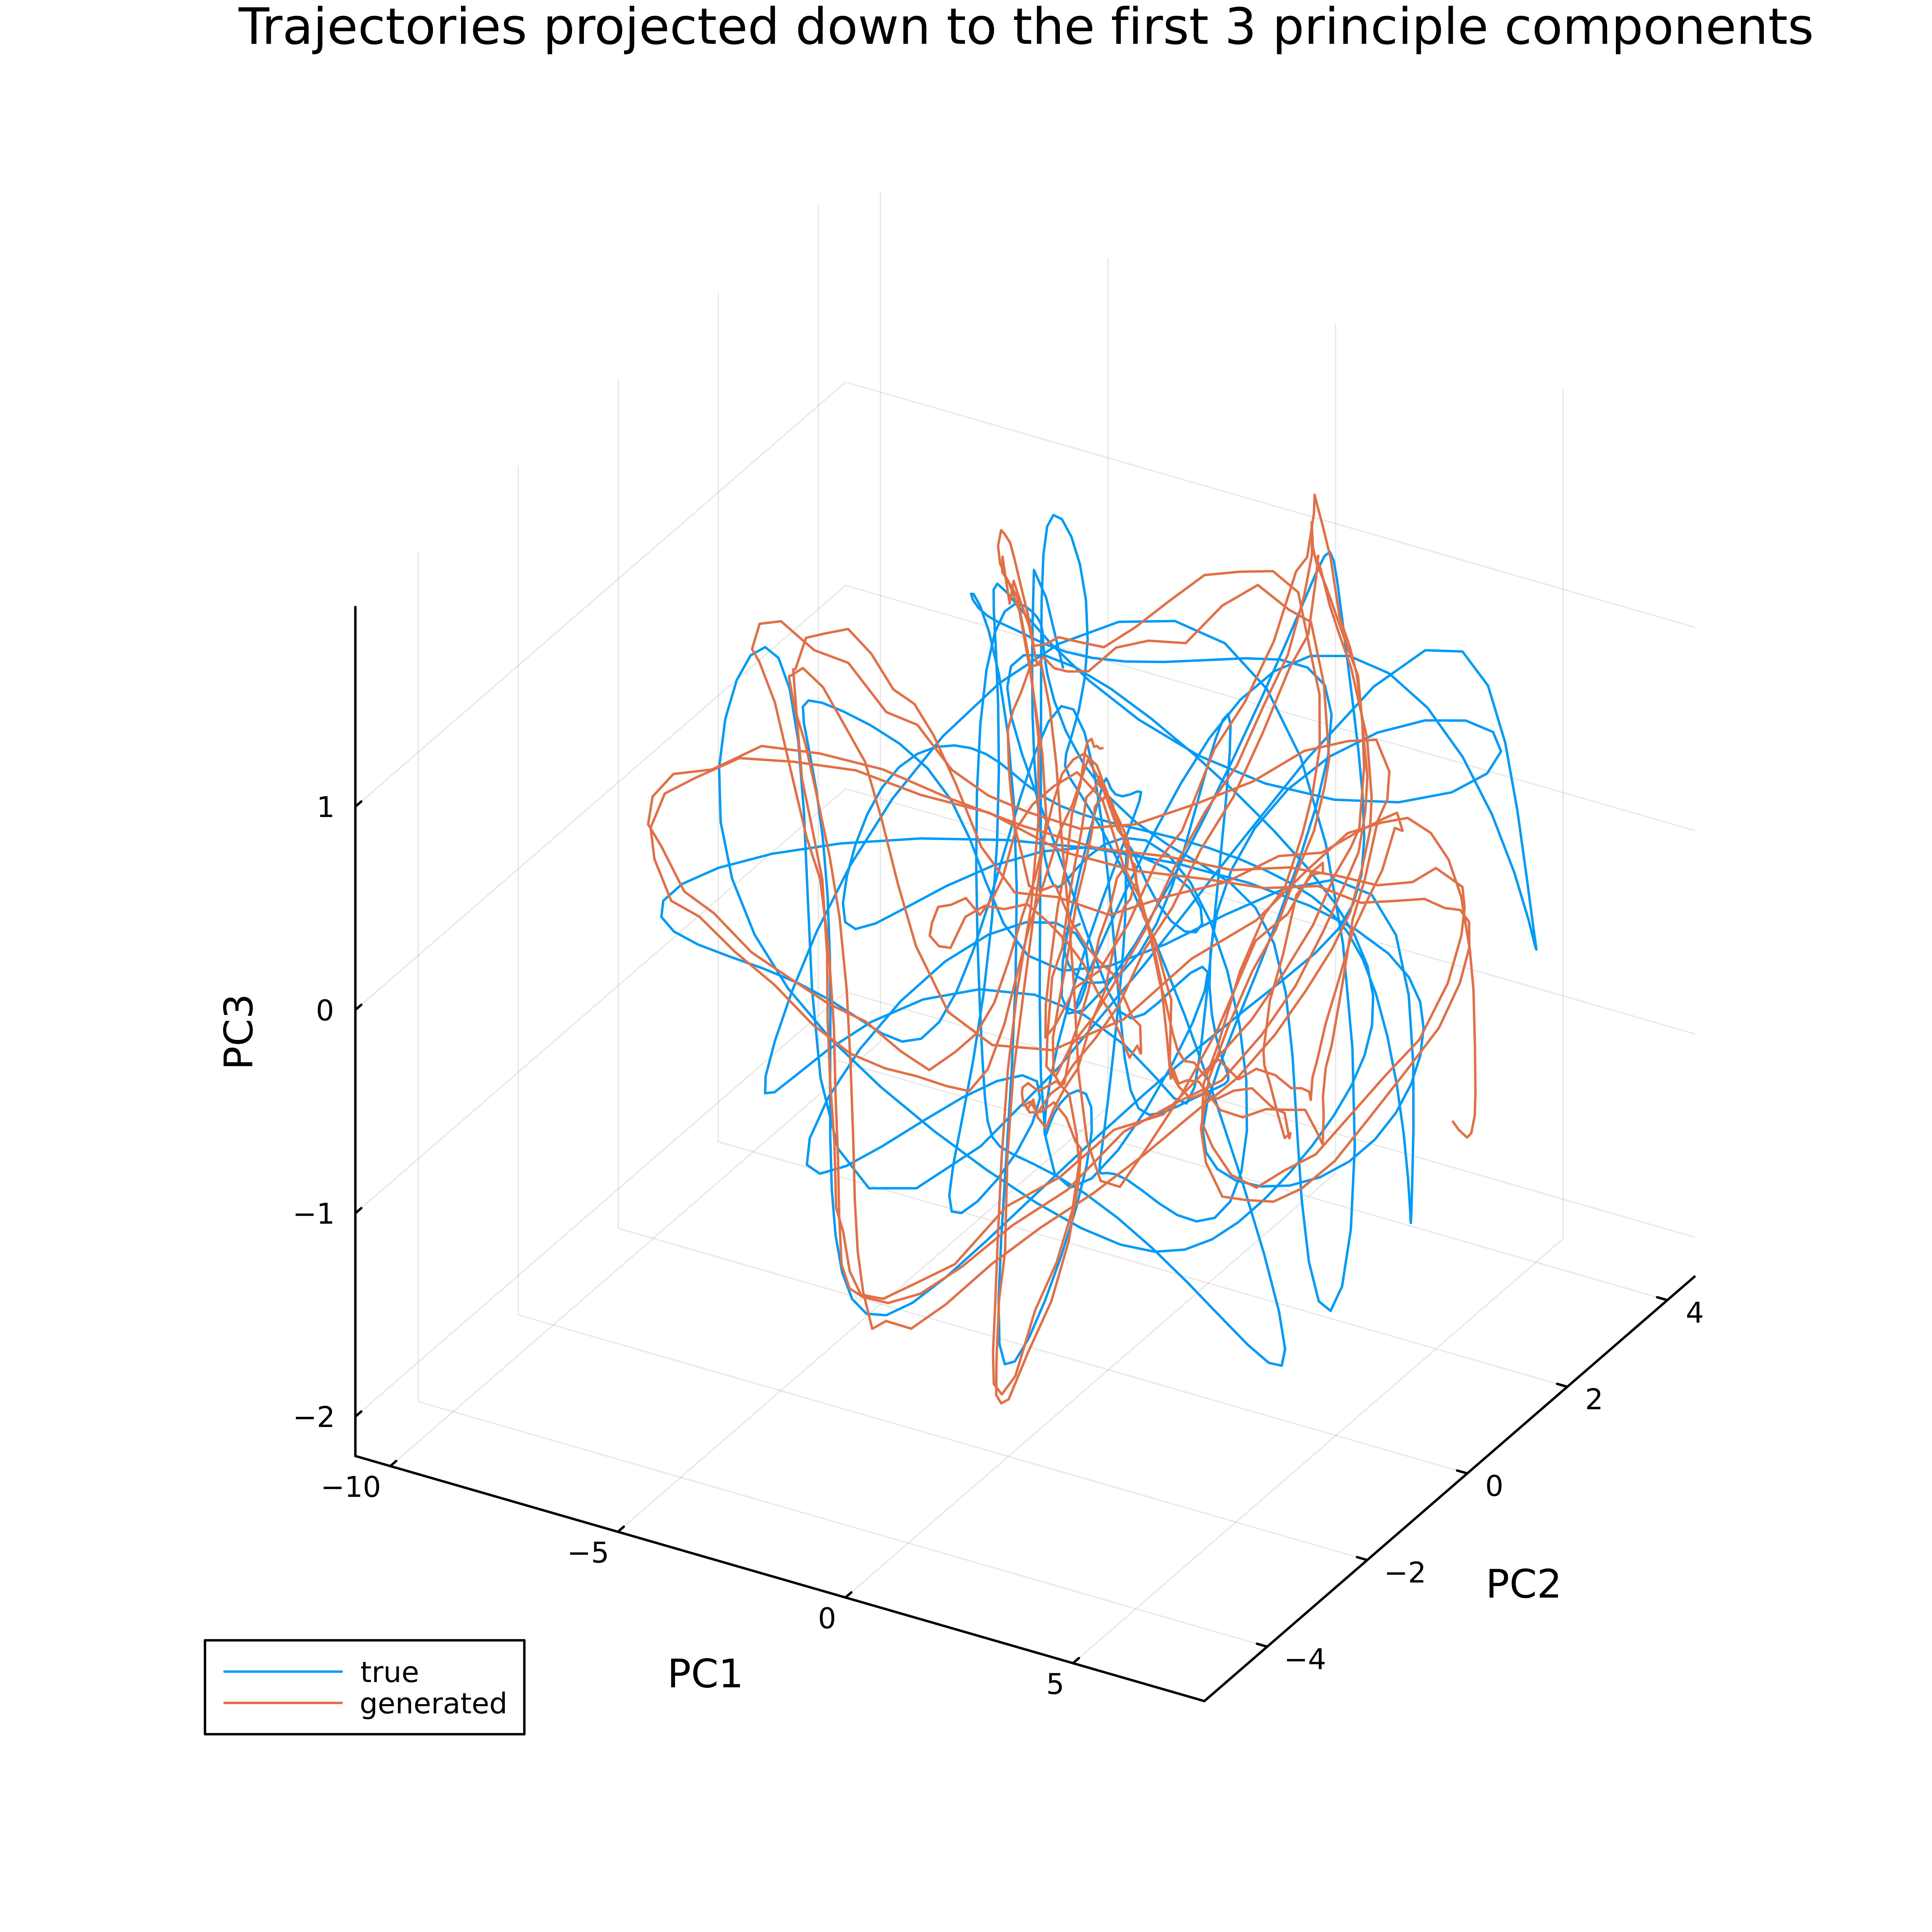
\includegraphics[width=\textwidth]{Images/pca_traj_reconstruction.png}
    \caption[Trajectories projected down to the first 3 principal components]
    {\textbf{Trajectories projected down to the first 3 principal components: } Trajectory generated by a model (\textit{orange}) compared to a real trajectory (\textit{blue}).
    The first 3 principal components of the true data are used.}
    \label{fig:pca_traj_reconstruction}
\end{figure}

When looking at different model runs it can be observed that a low $D_{stsp}$ value and a low $D_{PSE}$ often don't coincide.
In figure \ref{fig:metric_trajectory_comparison} I plotted some examples of trajectories with different combinations of high/low $D_{stsp}$ and $D_{pse}$ values to examine 
what these differences mean for the reconstruction.

\begin{figure}
    \includegraphics[width=\textwidth]{Images/metric_trajectory_comparison.png}
    \caption[Comparison of trajectories with different $D_{stsp}$ and $D_{PSE}$ combinations]
    {\textbf{Comparison of trajectories with different $D_{stsp}$ and $D_{PSE}$ combinations: } Trajectories and power spectra generated by models (\textit{orange}) with different 
    $D_{stsp}$ and $D_{PSE}$ values compared to the real trajectories (\textit{blue}).}
    \label{fig:metric_trajectory_comparison}
\end{figure}

From looking at the different examples shown in figure \ref{fig:metric_trajectory_comparison} it is immediately apparent that a high $D_{stsp}$ and $D_{PSE}$ result in 
a bad model which isn't able to reconstruct the dynamics at all. In the case of a low $D_{stsp}$ combined with a high $D_{PSE}$ the model is missing the dominant 
frequency of the participant data, which can be seen in the power spectrum. Instead, there is a peak at 0, meaning the model learned a constant offset instead of the 
dominant frequency of the training trajectory. The reconstructions with a low $D_{PSE}$ both look quite good as the dominant frequency is captured well and no artificial 
mode at 0 was learned. It is not apparent from the plot why $D_{stsp}$ is so high or what part of state space the model is not capturing. But considering that $D_{stsp}$ has 
a high variance in short trajectories, as noted in section \ref{sec:eval_metrics_param}, it seems that the power spectrum error $D_{PSE}$ is the more important and 
expressive metric for fMRI data.

\FloatBarrier
\subsection{Further investigation of dynamical features}

To further characterize the models, I calculated the Lyapunov spectrum (see section \ref{sec:lya_exp}) of the trained PLRNNs. The Lyapunov spectrum of a general RNN
can be calculated using the algorithm given in \cite{vogt2022lyapunov}. The mean and standard deviation of the maximum Lyapunov exponent $\lambda_{max}$ over all runs for 
each participant is shown in figure \ref{fig:max_le_of_patients}.

\begin{figure}
    
\includegraphics[width=\textwidth]{Images/max_le_of_patients.png}
    \caption[Maximum Lyapunov exponents estimated over all model runs]
    {\textbf{Maximum Lyapunov exponents estimated over all model runs: } $\lambda_{max}$ mean and standard deviation across model runs. Values of non-converged models were 
    excluded.}
    \label{fig:max_le_of_patients}
\end{figure}

Figure \ref{fig:max_le_of_patients} clearly shows that most of the models learn a positive $\lambda_{max}$ in training, i.e. chaotic dynamics. Only for a few participants, 
such as Nr. 282, are there several runs with an entirely negative Lyapunov spectrum. The models with negative Lyapunov spectrum typically performance issues if 
evolved freely over time. They either decay towards a constant value or they, at some point, fall into a simple oscillatory cycle. Examples of these behaviors are shown in 
figure \ref{fig:pos_neg_le_comparison} and figure \ref{fig:oscillator_neg_le}. These findings suggest that $\lambda_{max}$ needs to be taken into account when determining model 
quality. 

\begin{figure}
    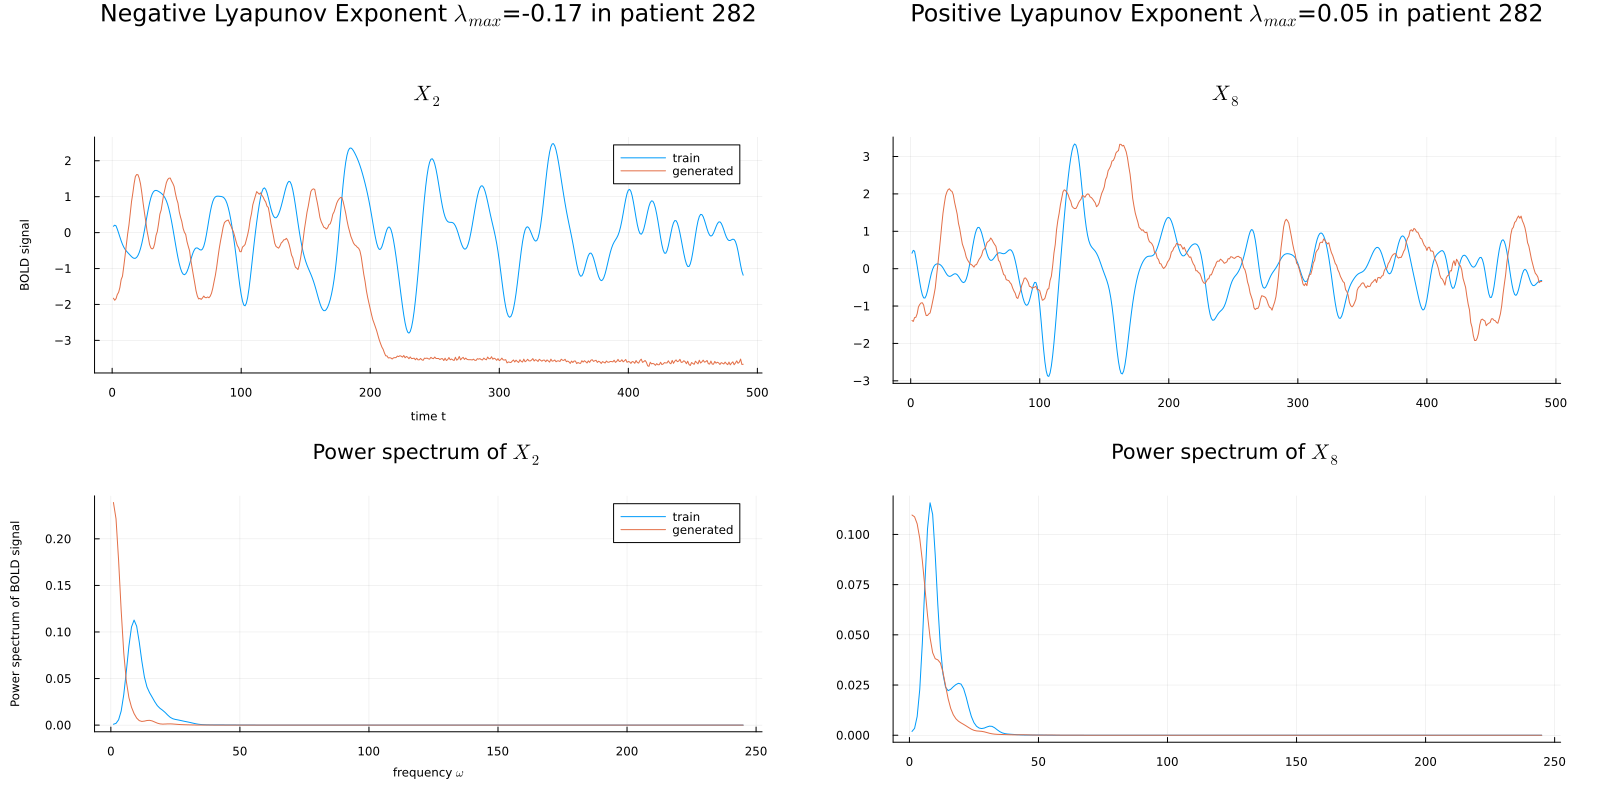
\includegraphics[width=\textwidth]{Images/pos_neg_le_comparison.png}
    \caption[Comparison between a model with positive and a model with negative $\lambda_{max}$]
    {\textbf{Comparison between a model with positive and a model with negative $\lambda_{max}$: } The model with a negative $\lambda_{max}$ simply decays towards a constant 
    value after initially producing a trajectory similar to the participant data. }
    \label{fig:pos_neg_le_comparison}
\end{figure}

\begin{figure}
    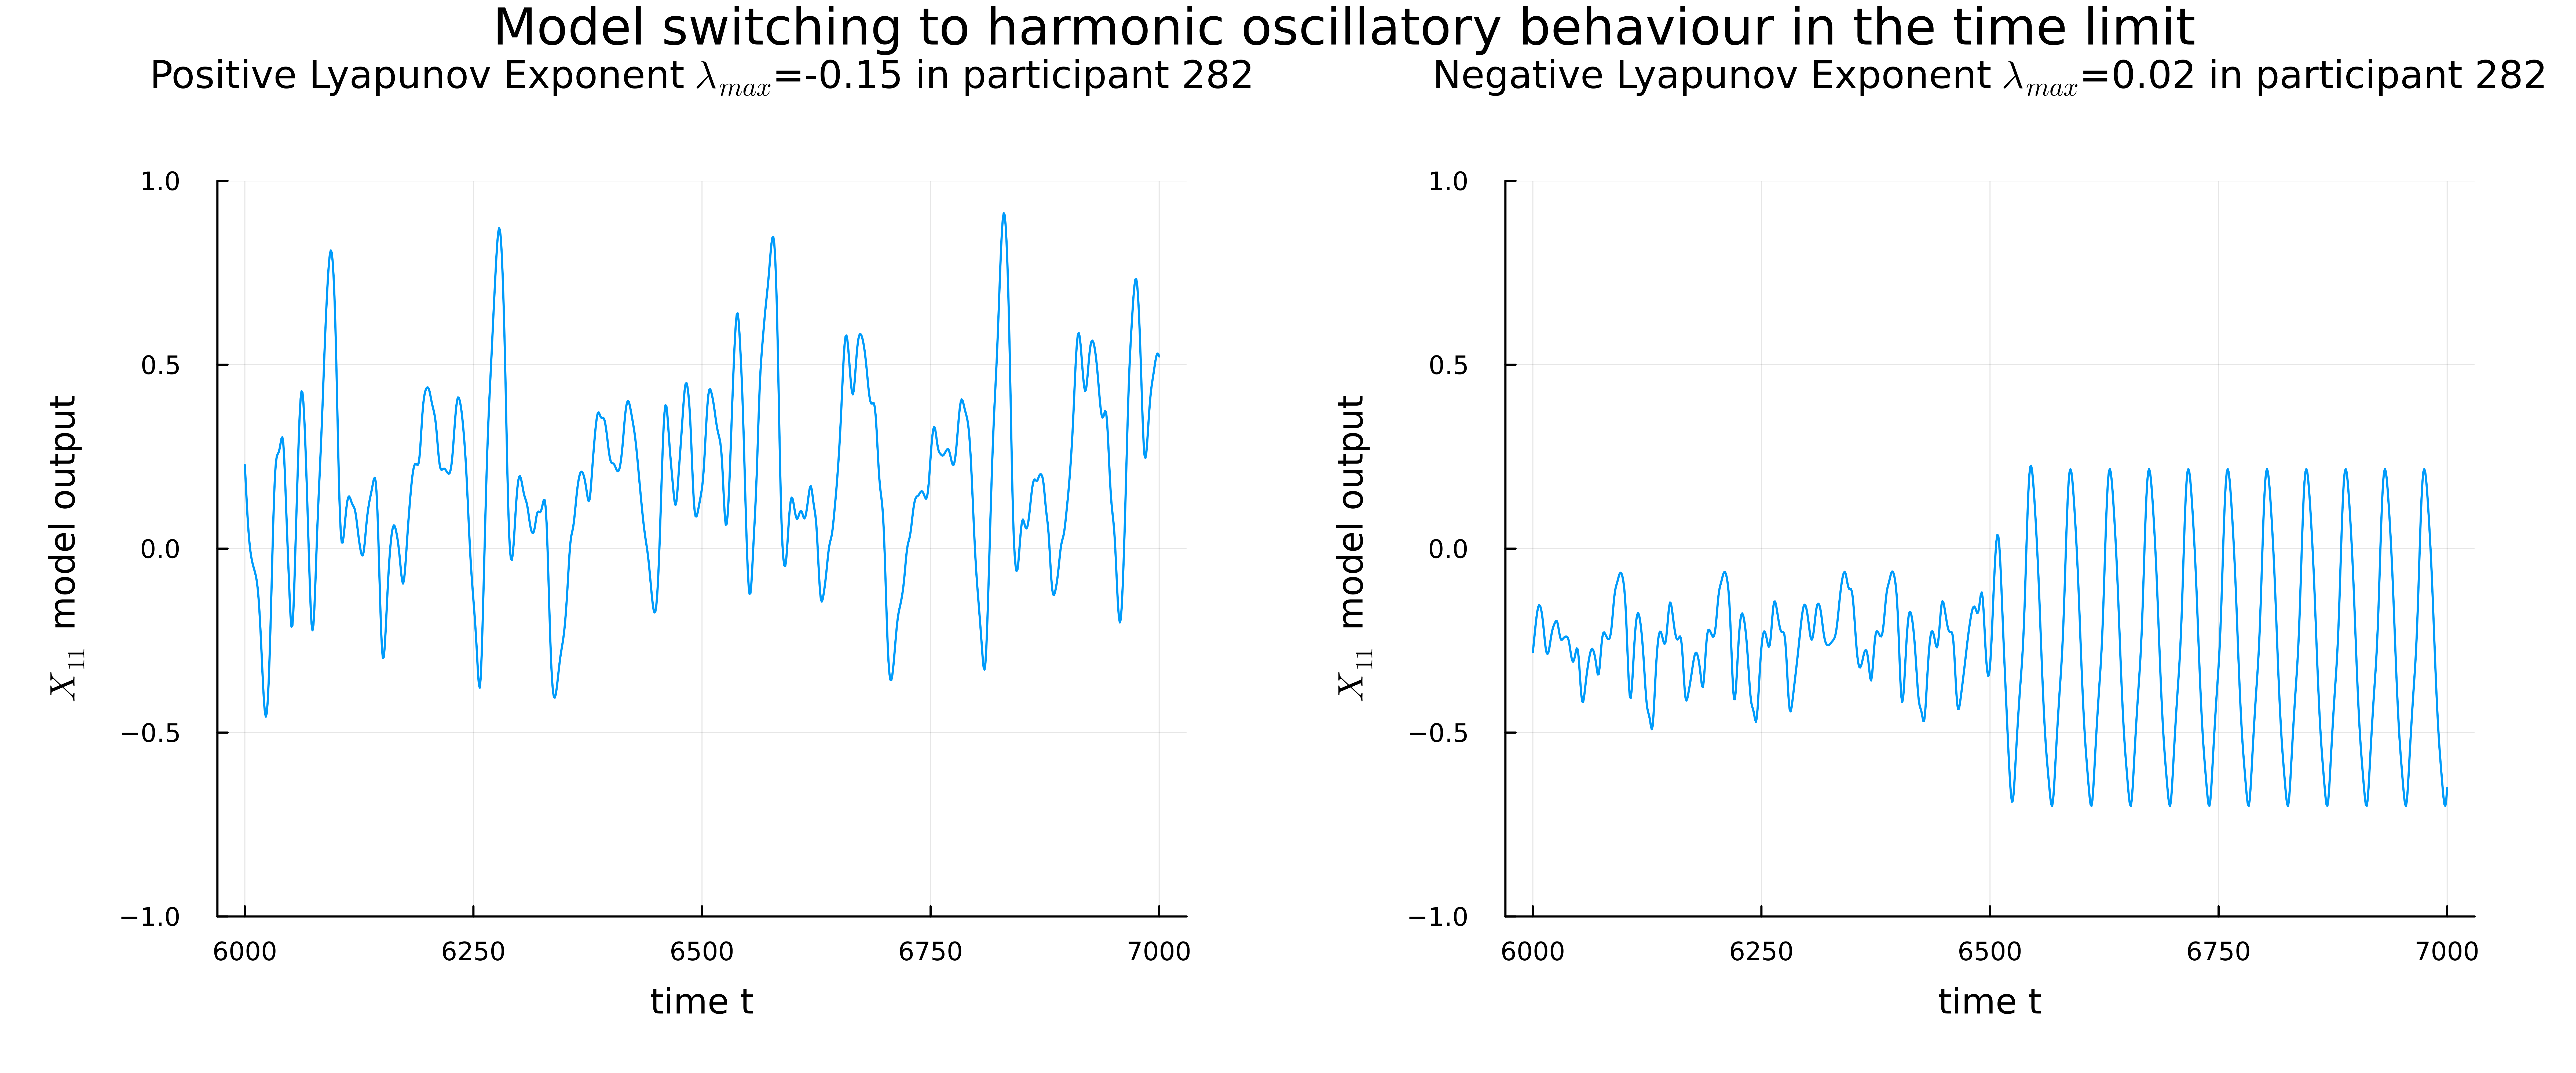
\includegraphics[width=\textwidth]{Images/oscillator_neg_le.png}
    \caption[Model switching to harmonic oscillatory behavior in the time limit]
    {\textbf{Model switching to harmonic oscillatory behavior in the time limit: } The model with a negative $\lambda_{max}$ simply switches to simple oscillations 
    after evolving freely for enough time steps. Note that this time is not fixed to the model. If initialized with a random state it may almost immediately exhibit this 
    behavior or only after many time steps as shown in the plots.}
    \label{fig:oscillator_neg_le}
\end{figure}

Similar to the maximum Lyapunov exponent I also examined the spectral norms of the $W_1$ and $W_2$ matrices of the trained models. The spectral norm of a matrix 
$\boldsymbol{A} \in \mathbb{R}^{M \times N}$ is induced by the $L_2$-norm and defined as 

\begin{equation}
    \| \boldsymbol{A} \|_2 = \max_{\|x\|_2=1} \|\boldsymbol{A} x \|_2 = \lambda_{max}(A^T A)
    \label{eq:spec_norm_def}
\end{equation}

where $\lambda_{max}(A^T A)$ is the maximum eigenvalue of $A^T A$. The mean and standard deviation of the W matrices spectral norms is shown in
figure \ref{fig:w_matrix_mean_std}. The matrix norms clearly vary much more between participants than the maximum Lyapunov exponent does. 

\begin{figure}
    \includegraphics[width=\textwidth]{Images/w_matrix_mean_std.png}
    \caption[Spectral norm of W matrices for each participant estimated over all model runs]
    {\textbf{Spectral norm of W matrices for each participant estimated over all model runs: } The spectral norm mean and standard deviation of the $W_1$ and $W_2$ matrices
    across model runs. Values of non-converged models were excluded.}
    \label{fig:w_matrix_mean_std}
\end{figure}

\FloatBarrier
\section{Investigating Correlations}

Next, I will investigate the correlations between the maximal Lyapunov exponents and W matrix spectral norms. In the following I use the Pearson correlation coefficient, which 
is defined as follows given a paired data sample $\left\{ (x_1, y_1), \cdots, (x_n, y_n) \right\}$:

\begin{equation}
    r_{x, y} = \frac{\text{CoV}(X, Y)}{\sqrt{\text{Var}(X)\text{Var}(Y)}} = \frac{\sum_{i=1}^{n}(x_i - \bar{x})(y_i - \bar{y})}{\sqrt{\sum_{i=1}^{n}(x_i - \bar{x})} \sqrt{\sum_{i=1}^{n}(y_i - \bar{y})}}
    \label{eq:cor_coef_def}
\end{equation}

where $\bar{x}$ and $\bar{y}$ are the respective sample means (\cite{mcdonald2014handbook}). The elements of the correlation matrices shown in the following 
are the pairwise correlation coefficients $r_{ij} = \frac{\text{CoV}(X_i, X_j)}{\sqrt{\text{Var}(X_i)\text{Var}(X_j)}}$ of the elements of the 
random vector $X = \left(X_1, \cdots, X_n\right)$.

I plotted correlation matrices of the maximal Lyapunov exponents in figure \ref{fig:corr_matrix_max_le} and in figure \ref{fig:corr_matrix_max_le_filtered}. What is shown are the 
correlations between runs across all participants. In the figure \ref{fig:corr_matrix_max_le} all runs are included except for not converged runs. Because there are up to 2 non-converged
runs per participant, I reordered the runs such that non-converged runs are indexed as runs 19 and 20 and excluded these rows and columns from the plots as they included NaNs/missing 
entries to calculate the statistics. The remaining model runs are ordered by sorting from lowest to highest $D_{PSE}$,
i.e. the run with the lowest $D_{PSE}$ is run 1, second lowest is run 2 etc. Because the run number/index is arbitrary this reordering 
does not make any differences in the results, only for the position on the matrix.

In the figure \ref{fig:corr_matrix_max_le_filtered} I filtered the runs to only include the best models based on the $D_{stsp}$ and $D_{PSE}$ metrics. To be precise,
I filtered the runs by first selecting the models with the 10 best $D_{stsp}$ scores and then further filtered those 10 by only selecting the 5 models with the best $D_{PSE}$ results.
This results in 5 runs per participants which are indexed by sorting from best to worst $D_{PSE}$ as in the previous correlation matrix.

The correlations are mostly weak and positive, as indicated by the heatmap coloring of the matrix entries. The idea behind the filtering was that the image would be decisively 
different by only including good models and only the stronger correlations would remain in the filtered matrix. This is not the case and the few stronger correlations in 
figure \ref{fig:corr_matrix_max_le} are no longer presence in figure \ref{fig:corr_matrix_max_le_filtered}. The negative correlations are almost entirely eliminated up to 
one entry very close to zero (-0.045).

I repeated the identical process for the spectral norms of the $W_1$ and $W_2$ matrices. The unfiltered correlation matrices are shown in figure \ref{fig:corr_matrix_w_spec_norm},
the filtered correlation matrices are shown in figure \ref{fig:corr_matrix_spec_norms_filtered}. The results here are similar, mostly weak positive correlations in the unfiltered
matrices. In the filtered matrices all negative correlations are eliminated.

\begin{figure}
    \begin{subfigure}[t]{0.48\textwidth}
        \centering
        \includegraphics[width=\textwidth]{Images/corr_matrix_max_le.png}
        \caption[Correlation matrix of maximum Lypunov exponent over all converged runs]
        {\textbf{Correlation matrix of maximum Lypunov exponent over all converged model runs: } Because there are up to 2 not converged model runs per participant the runs were 
        reordered such that the not converged runs are at position 19 and 20 and left out of the correlation matrix. Runs arranged in ascending order by $D_{PSE}$}
        \label{fig:corr_matrix_max_le}
    \end{subfigure}
    \begin{subfigure}[t]{0.48\textwidth}
        \centering
        \includegraphics[width=\textwidth]{Images/corr_matrix_max_le_filtered.png}
        \caption[Correlation matrix of maximum Lypunov exponent over filtered model runs]
        {\textbf{Correlation matrix of maximum Lypunov exponent over filtered model runs: } Model runs were filtered by first selecting the runs with the lowest 10 $D_{stsp}$.
        Then the runs with the lowest 5 $D_{PSE}$ are selected of those 10. Runs arranged in ascending order by $D_{PSE}$}
        \label{fig:corr_matrix_max_le_filtered}
    \end{subfigure}
    \caption[Correlation matrices of the maximum Lypunov exponents]{Correlation matrices of the maximum Lypunov exponents}
    \label{fig:max_le_cor_matrices}
\end{figure}

\begin{figure}
    \includegraphics[width=\textwidth]{Images/corr_matrix_w_spec_norm.png}
    \caption[Correlation matrices of W matrices spectral norms over all model runs]
    {\textbf{Correlation matrices of W matrices spectral norms over all model runs: } Because there are up to 2 not converged model runs per participant the runs were 
    reordered such that the not converged runs are at position 19 and 20 and left out of the correlation matrix. Runs arranged in ascending order by $D_{PSE}$}
    \label{fig:corr_matrix_w_spec_norm}
\end{figure}

\begin{figure}
    \includegraphics[width=\textwidth]{Images/corr_matrix_spec_norms_filtered.png}
    \caption[Correlation matrices of W matrices spectral norms over filtered model runs]
    {\textbf{Correlation matrices of W matrices spectral norms over filtered model runs: } Model runs were filtered by first selecting the runs with the lowest 10 $D_{stsp}$.
    Then the runs with the lowest 5 $D_{PSE}$ are selected of those 10. Runs arranged in ascending order by $D_{PSE}$.}
    \label{fig:corr_matrix_spec_norms_filtered}
\end{figure}

To conclude this work, I lastly searched for correlations between the dynamical features of the trained models and measurable traits of the participants. The different 
rs-fMRI frequency bands have been linked to personality traits, see \cite{ikeda2017comprehensive} and \cite{dubois2018resting}, which find a connection between 
the traits Openness and Extraversion to analyzed rs-fMRI data. I calculated the mean maximum Lyapunov exponents for all participants, once over all converged models and
then only over 5 best models (so same filtering as before) and correlated these with different personality measures. The personality measures are selection of those 
included in the LEMON dataset. I used the State-Trait Anxiety Inventory \cite{spielberger1970manual}, the Hamilton rating scale for depression \cite{hamilton1960rating}, 
and the big 5 personality traits \cite{costa1989neo}. Because not all participants are included in every personality measure I added the number of participants $N_{participants}$
for which data was available to the results. It should be noted that in this analysis, no correction for multiple testing was performed.

The results for the unfiltered exponents are shown in table \ref{tab:mean_le_personality_cor_table}, the results for the filtered exponents in
table \ref{tab:mean_le_filtered_personality_cor_table}. There are no significant correlations. 

\begin{table}
\centering
\caption{Correlation between personality measures and mean maximum Lyapunov exponents. Mean $\lambda_{max}$                                                                                   is calculated from all converged models. The results are statistically significant at a p-value$<0.05$.                                                                                   No correction for multiple testing was performed.}
\label{tab:mean_le_personality_cor_table}
\begin{tabular}{lllll}
\toprule
 & $N_{Participants}$ & Correlation & p-Value & Significant \\
Personality Scale &  &  &  &  \\
\midrule
STAI Anxiety & 50 & -0.093 & 0.519 & False \\
Hamilton Depression scale & 50 & 0.148 & 0.306 & False \\
Neuroticism & 50 & -0.025 & 0.864 & False \\
Extraversion & 50 & -0.053 & 0.716 & False \\
Openness For Experiences & 50 & -0.275 & 0.053 & False \\
Agreeableness & 50 & 0.075 & 0.605 & False \\
Conscientiousness & 50 & -0.016 & 0.911 & False \\
\bottomrule
\end{tabular}
\end{table}

\begin{table}
\centering
\caption{Correlation between personality measures and mean maximum Lyapunov exponents. Mean $\lambda_{max}$                                                                                   is only calculated from filtered models. The results are statistically significant at a p-value$<0.05$.                                                                                   No correction for multiple testing was performed.}
\label{tab:mean_le_filtered_personality_cor_table}
\begin{tabular}{lllll}
\toprule
 & $N_{Participants}$ & Correlation & p-Value & Significant \\
Personality Scale &  &  &  &  \\
\midrule
STAI Anxiety & 50 & 0.053 & 0.716 & False \\
Hamilton Depression scale & 50 & 0.127 & 0.381 & False \\
Neuroticism & 50 & 0.026 & 0.860 & False \\
Extraversion & 50 & 0.057 & 0.695 & False \\
Openness For Experiences & 50 & 0.038 & 0.793 & False \\
Agreeableness & 50 & 0.039 & 0.789 & False \\
Conscientiousness & 50 & -0.094 & 0.518 & False \\
\bottomrule
\end{tabular}
\end{table}
